% ============================================================
% 电路基础实验 —— 实验一 电路基本概念与定律 实验报告
% 使用 CircuitTheory/template.tex 正式实验报告模板
% ============================================================

\documentclass[12pt]{ctexart}

% --- 宏包 ---
\usepackage{graphicx}
\usepackage{amsmath}
\usepackage{float}
\usepackage{booktabs}
\usepackage{siunitx}
\usepackage{caption}
\usepackage{subcaption}
\usepackage{enumitem}
\usepackage{fancyhdr}
\usepackage{hyperref}
\usepackage{makecell}

\sisetup{per-mode=symbol}

\graphicspath{{./figure/}{./figures/}{../}{../requirements/extracted_images/word/media/}{./}}

\usepackage[left=2.5cm, right=2.5cm, top=2.5cm, bottom=2.5cm]{geometry}

\setlength{\jot}{6pt}
\setlength{\headheight}{15pt}
\linespread{1.5}
\setlist{nosep}

% --- 页眉页脚 ---
\pagestyle{fancy}
\fancyhead[C]{电路基础实验}
\fancyfoot[C]{\thepage}

\begin{document}

% ==================== 封面 ====================
\thispagestyle{empty}

\begin{figure}[t]
    \centering
    
\includegraphics[width=13cm]{logo1.png}
\end{figure}

\vspace*{\fill}
    \begin{center}
        \Huge\textbf{电路基础}

        \vspace{0.3cm}
        \Huge\textbf{实验报告}

        \vspace{1cm}
        \LARGE\textbf{实验一：电路基本概念与定律}
    \end{center}
\vspace*{\fill}

\begin{table}[H]
    \centering
    \large
    \begin{tabular}{ll}
    \toprule
    \textbf{课程:} & 电路基础实验 \\
    \textbf{姓名:} & 郭浩然 2024303980 \\
    \textbf{组号:} & 第7组 \\
    \textbf{时间:} & \today \\
    \bottomrule
    \end{tabular}
\end{table}

\newpage

% ==================== 正文 ====================

% (10) 1、实验目的
\section{实验目的}

\begin{enumerate}[label=\arabic*.]
    \item 学习使用数字万用表测量电阻阻值、电压和电流的方法。
    \item 掌握直流电阻网络在面包板上的搭建与检查方法。
    \item 通过实测节点电流验证基尔霍夫电流定律（KCL）。
    \item 通过实测回路电压验证基尔霍夫电压定律（KVL）。
\end{enumerate}

% (20) 2、实验原理
\section{实验原理}

\subsection{基尔霍夫电流定律}

基尔霍夫电流定律指出，在集总参数电路中，任意节点在任意时刻流入该节点的电流代数和恒等于零。若约定流入节点的电流为正、流出节点的电流为负，则有
\begin{equation}
    \sum_{k=1}^{n} i_k = 0.
\end{equation}
该定律反映了电荷守恒关系。实验中选取电路中的一个节点，分别测量与该节点相连支路的电流，并计算电流代数和，以验证 KCL。

\subsection{基尔霍夫电压定律}

基尔霍夫电压定律指出，在集总参数电路中，任意闭合回路中各支路电压升与电压降的代数和恒等于零。若沿选定回路方向列写电压，则有
\begin{equation}
    \sum_{k=1}^{n} u_k = 0.
\end{equation}
该定律反映了能量守恒关系。实验中按照选定回路方向测量各电阻两端电压和电源电压，并计算回路电压代数和，以验证 KVL。

\subsection{实验电路与仿真}

实验电路由两个直流电压源和五个电阻组成，其中电阻标称值为 \(R_1=510\,\Omega\)、\(R_2=100\,\Omega\)、\(R_3=100\,\Omega\)、\(R_4=1\,\mathrm{k}\Omega\)、\(R_5=200\,\Omega\)。实验前使用 Multisim 搭建仿真电路，如图~\ref{fig:multisim} 所示，用于明确电路连接关系、测量对象和参考方向。

\begin{figure}[H]
    \centering
    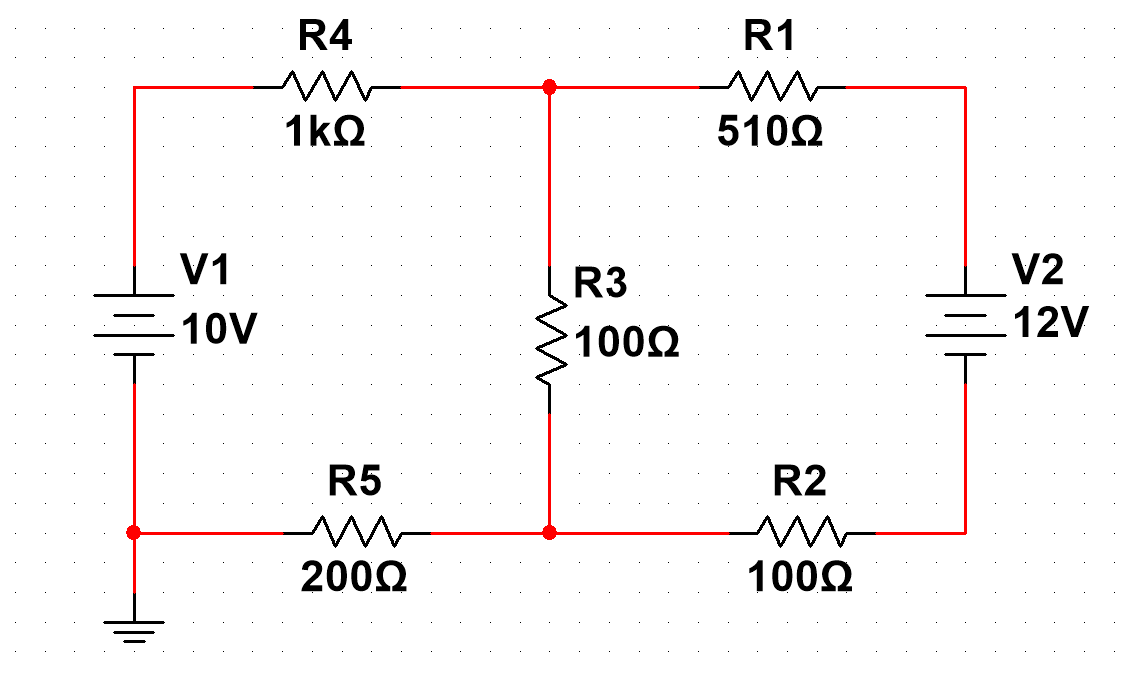
\includegraphics[width=0.88\textwidth]{image2.png}
    \caption{实验一 Multisim 仿真电路}
    \label{fig:multisim}
\end{figure}

% (10) 3、实验器件
\section{实验器件}

\begin{itemize}
    \item 面包板 \(\times 1\)
    \item 可编程直流电源 \(\times 1\)
    \item 数字万用表 \(\times 1\)
    \item 电阻：\(100\,\Omega\times 2\)、\(200\,\Omega\times 1\)、\(510\,\Omega\times 1\)、\(1\,\mathrm{k}\Omega\times 1\)
    \item 导线若干
\end{itemize}

% (10) 4、实验步骤
\section{实验步骤}

\begin{enumerate}[label=\arabic*.]
    \item 根据实验电路图选择所需电阻，并使用数字万用表电阻档测量各电阻的实际阻值。
    \item 使用万用表通断档检查导线是否导通，避免因导线或面包板接触不良影响实验结果。
    \item 按 Multisim 仿真电路在面包板上搭建实际电路，检查电源极性、公共节点和各电阻连接是否正确。
    \item 接入直流电源，设置电源电压，通电前再次检查电路连接，确认无短路风险。
    \item 使用万用表电压档测量 \(R_1\) 至 \(R_5\) 两端电压，并按统一参考方向记录正负号。
    \item 选取一个节点，使用万用表电流档测量该节点相连支路电流，并按流入节点为正的约定记录。
    \item 整理电阻、电压和电流数据，计算 KVL 回路电压代数和与 KCL 节点电流代数和。
\end{enumerate}

\begin{figure}[H]
    \centering
    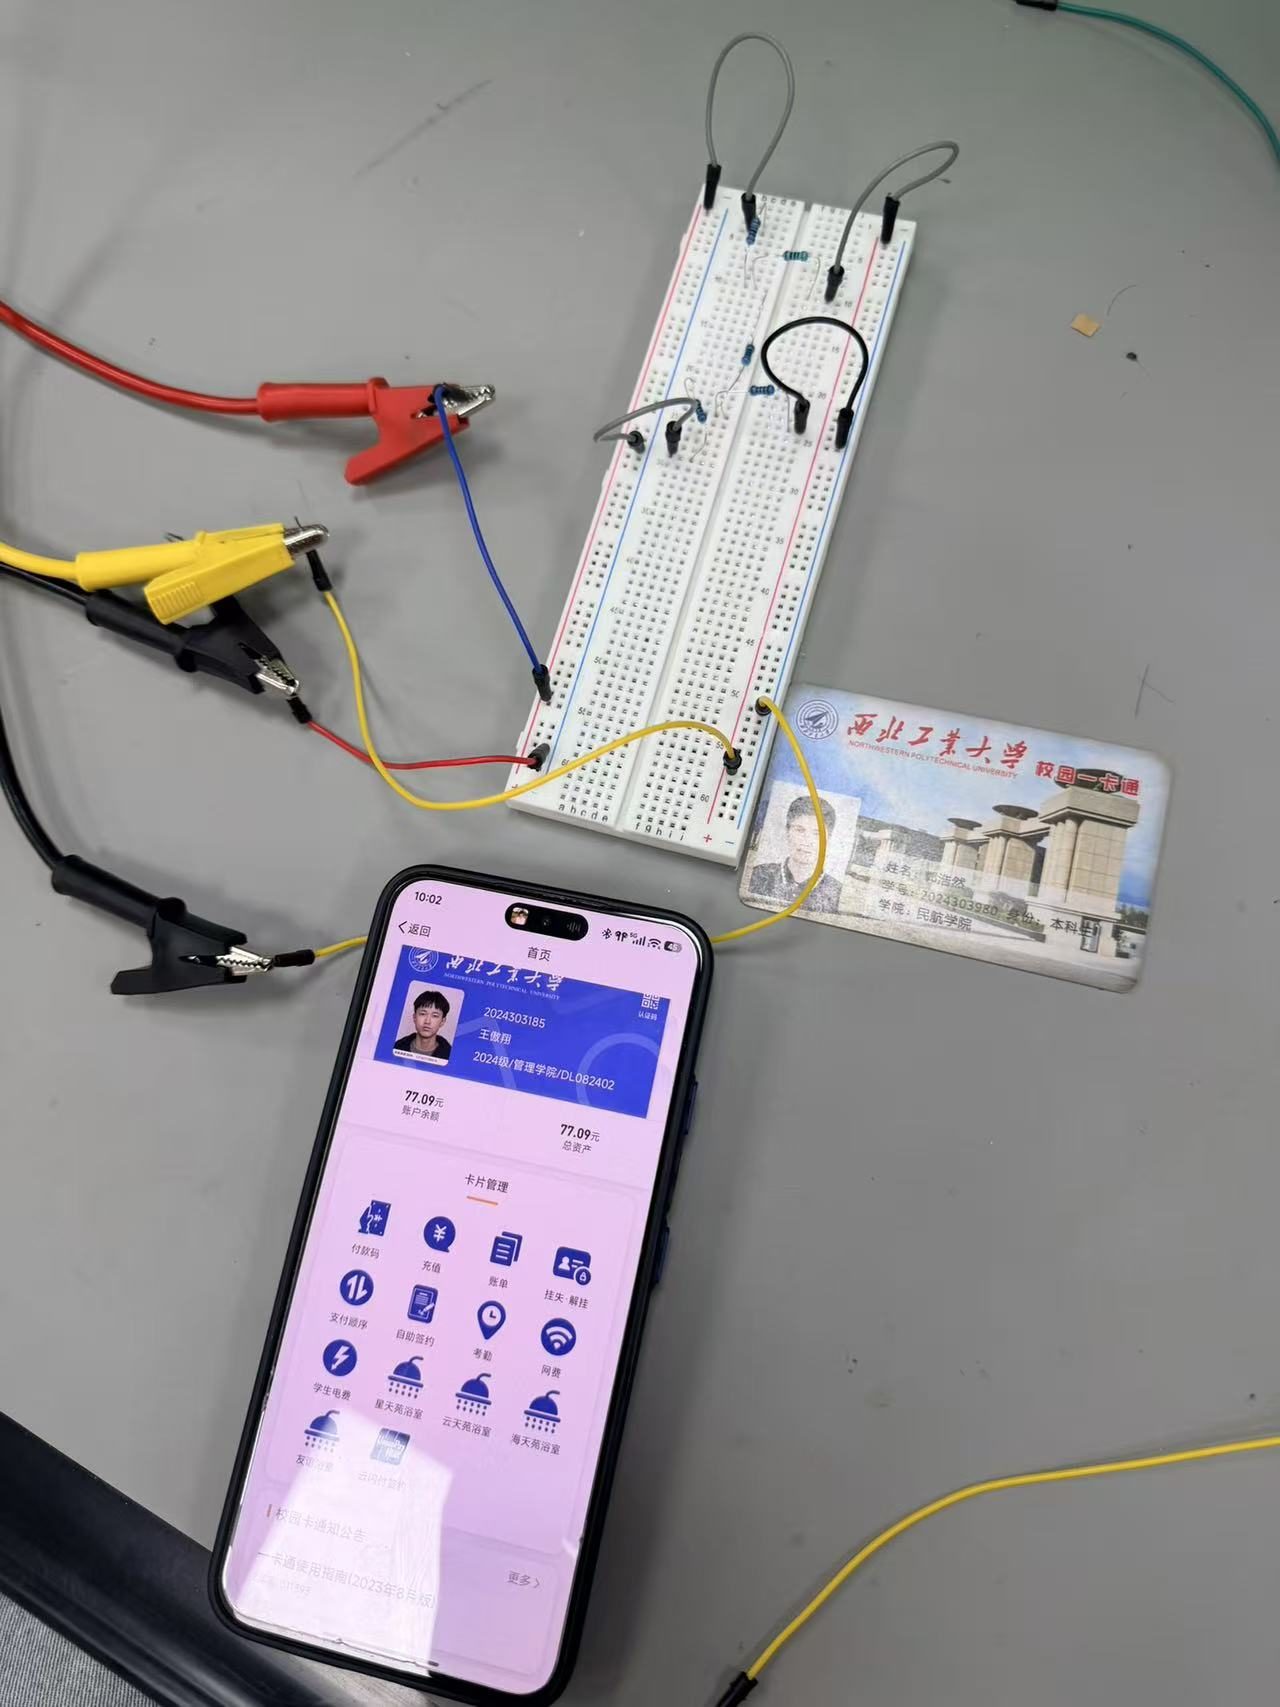
\includegraphics[width=0.55\textwidth]{实验1实物.jpg}
    \caption{实验一实物电路连接}
    \label{fig:physical-circuit}
\end{figure}

% (10) 5、实验数据
\section{实验数据}

实验原始数据记录如图~\ref{fig:raw-data} 所示。根据原始记录，将电阻实测值、电压测量值和电流测量值整理为表~\ref{tab:resistors} 至表~\ref{tab:kcl}。

\begin{figure}[H]
    \centering
    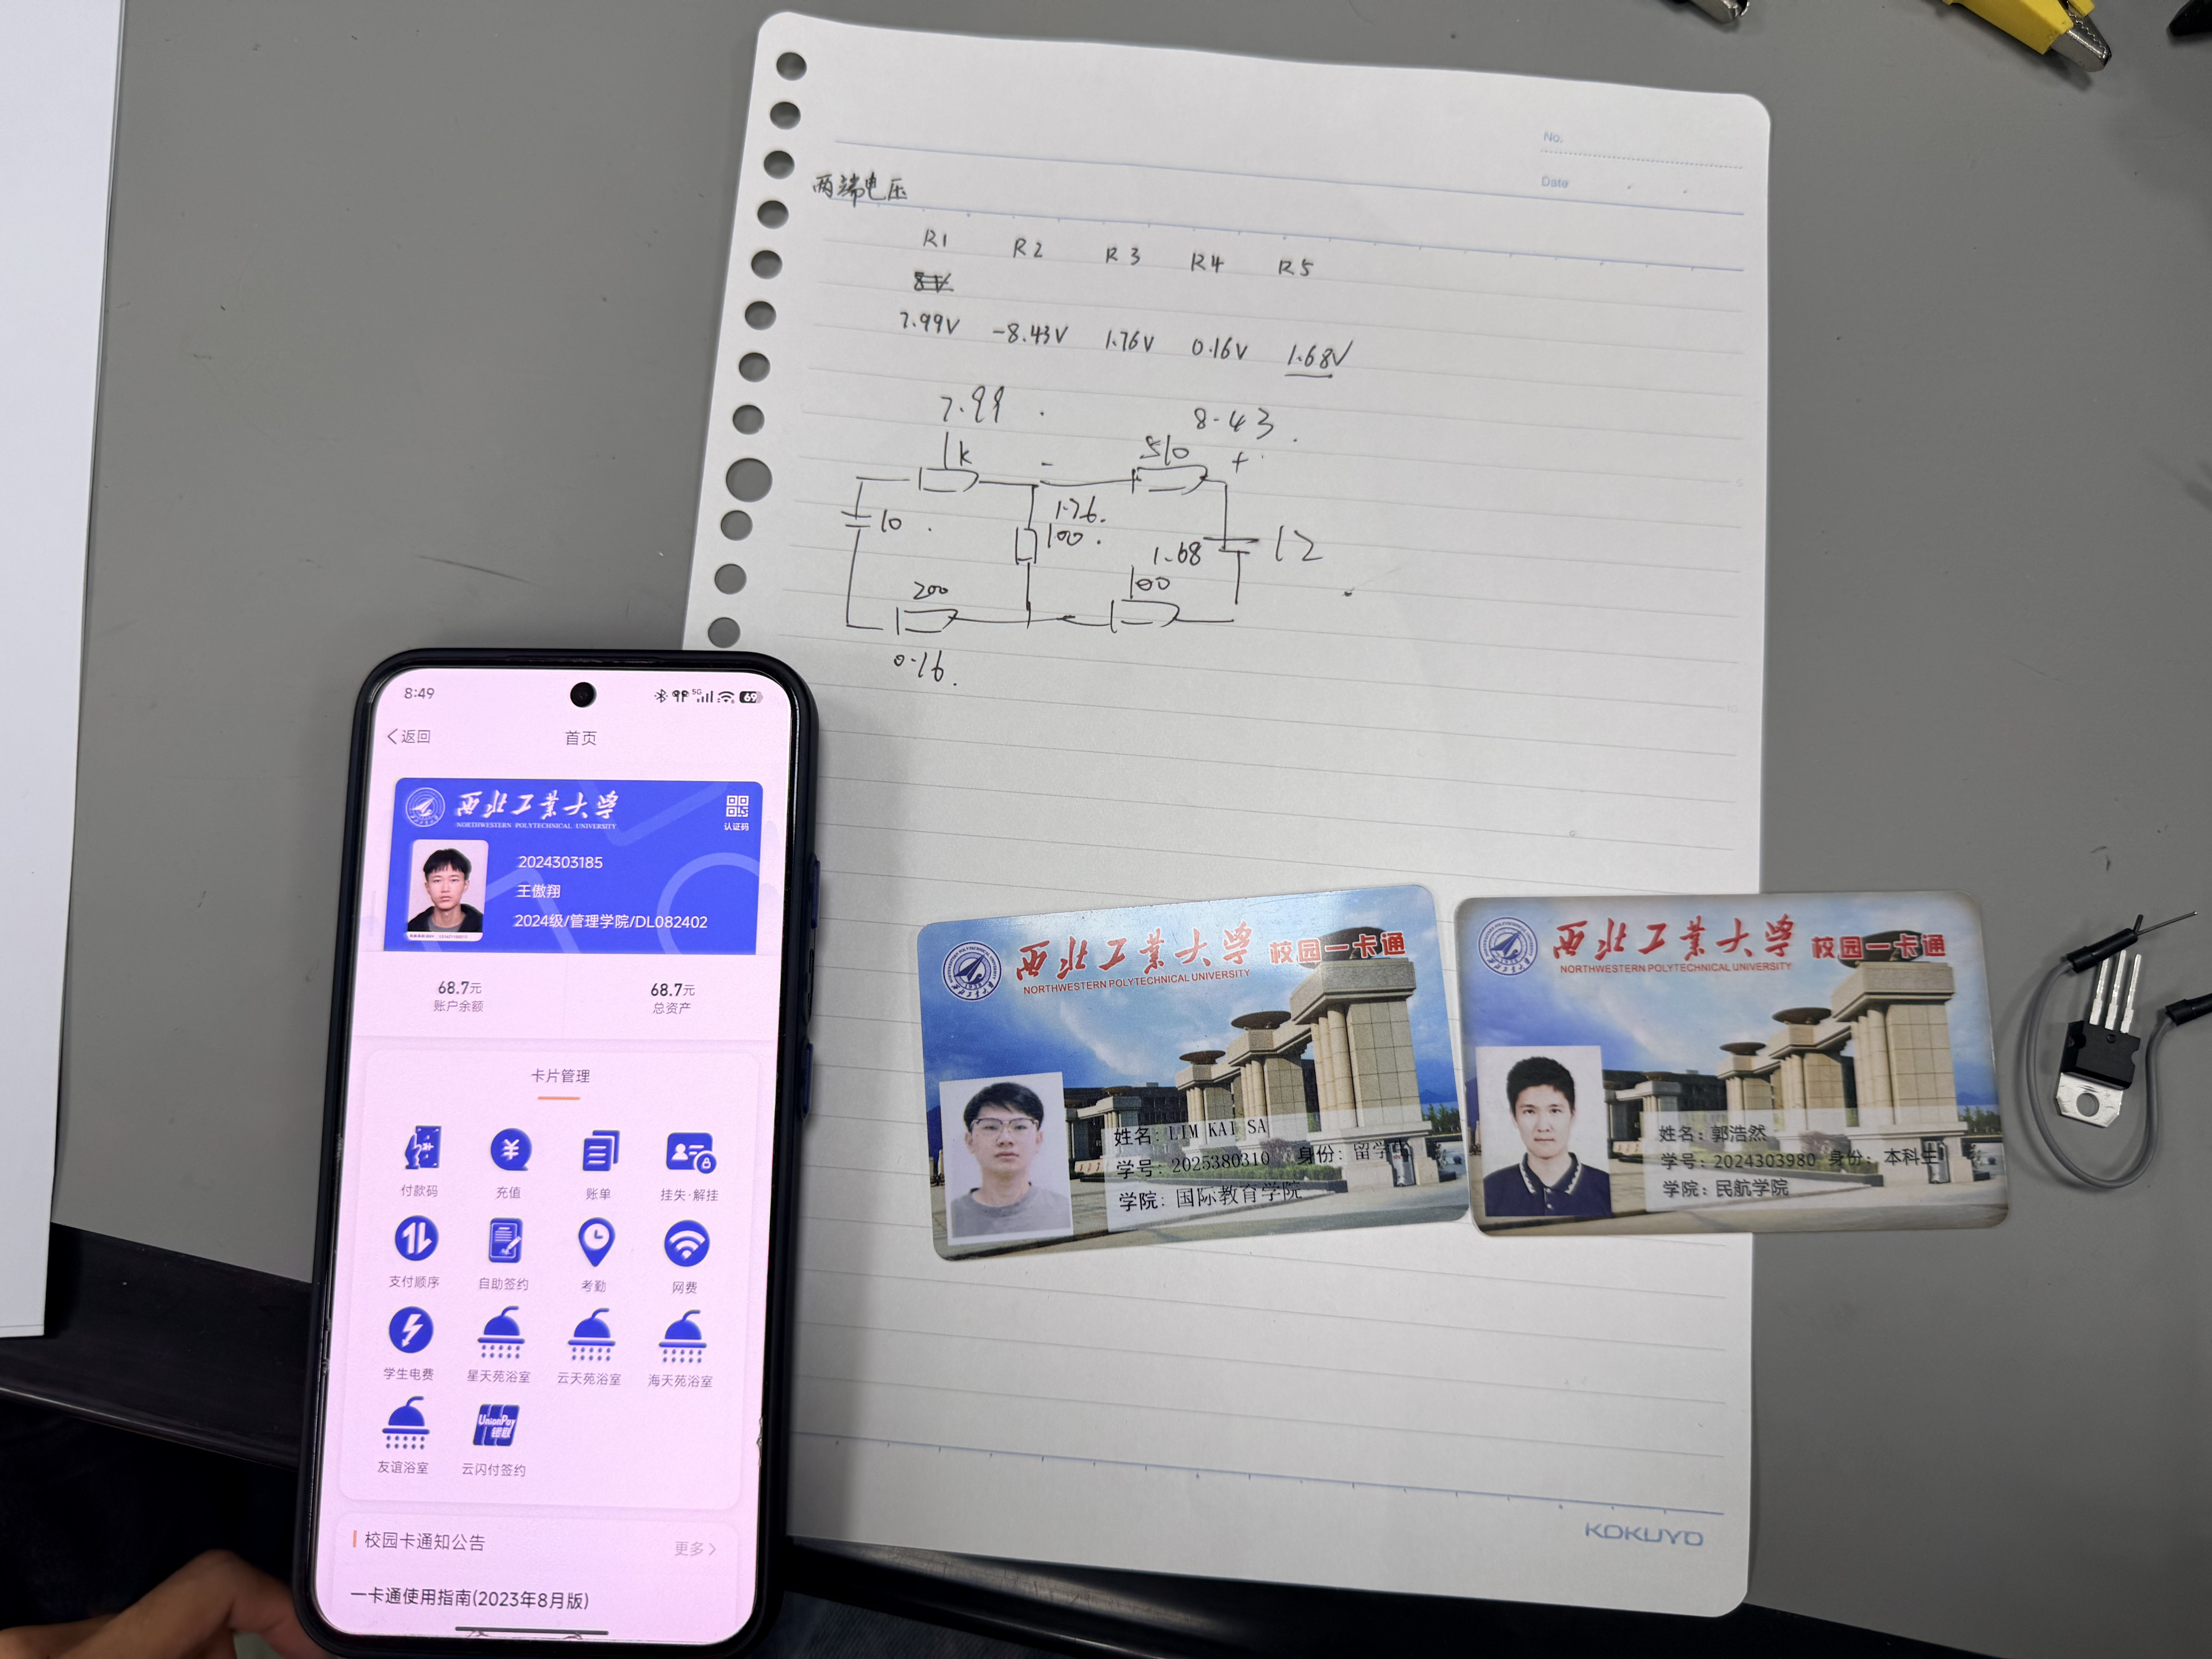
\includegraphics[width=0.82\textwidth]{实验1数据.jpg}
    \caption{实验一原始数据记录照片}
    \label{fig:raw-data}
\end{figure}

\begin{table}[H]
    \centering
    \caption{电阻实测值}
    \label{tab:resistors}
    \begin{tabular}{cccc}
        \toprule
        电阻 & 标称值/\(\Omega\) & 实测值/\(\Omega\) & 相对误差 \\
        \midrule
        \(R_1\) & 510 & 505.38 & 0.91\% \\
        \(R_2\) & 100 & 98.34 & 1.66\% \\
        \(R_3\) & 100 & 98.40 & 1.60\% \\
        \(R_4\) & 1000 & 994.20 & 0.58\% \\
        \(R_5\) & 200 & 196.00 & 2.00\% \\
        \bottomrule
    \end{tabular}
\end{table}

\begin{table}[H]
    \centering
    \caption{KVL 电压测量数据}
    \label{tab:kvl-voltage}
    \begin{tabular}{ccc}
        \toprule
        测量量 & 测量值/V & 说明 \\
        \midrule
        \(U_1\) & 8.149 & \(R_1\) 两端电压 \\
        \(U_2\) & 1.597 & \(R_2\) 两端电压 \\
        \(U_3\) & 2.237 & \(R_3\) 两端电压 \\
        \(U_4\) & -6.477 & \(R_4\) 两端电压 \\
        \(U_5\) & -1.280 & \(R_5\) 两端电压 \\
        \bottomrule
    \end{tabular}
\end{table}

\begin{table}[H]
    \centering
    \caption{KVL 验证结果}
    \label{tab:kvl}
    \begin{tabular}{ccc}
        \toprule
        回路 & 计算式 & 代数和/V \\
        \midrule
        回路一 & \(U_1+U_2+U_3-12\) & -0.017 \\
        回路二 & \(-U_3+U_4+U_5+10\) & 0.006 \\
        \bottomrule
    \end{tabular}
\end{table}

\begin{table}[H]
    \centering
    \caption{KCL 电流测量与验证结果}
    \label{tab:kcl}
    \begin{tabular}{ccc}
        \toprule
        测量量 & 测量值/mA & 说明 \\
        \midrule
        \(I_1\) & 16.139 & 流入节点为正 \\
        \(I_4\) & 6.506 & 流入节点为正 \\
        \(I_3\) & -22.554 & 流出节点记为负 \\
        \midrule
        \multicolumn{2}{c}{\(I_1+I_4+I_3\)} & 0.091 \\
        \bottomrule
    \end{tabular}
\end{table}

% (20) 6、数据分析
\section{数据分析}

\subsection{实验数据与理论公式对比}

由表~\ref{tab:kvl} 可知，回路一的电压代数和为 \(-0.017\,\mathrm{V}\)，回路二的电压代数和为 \(0.006\,\mathrm{V}\)，均接近零。与 KVL 理论式 \(\sum u_k=0\) 相比，实测偏差很小，说明在实验误差允许范围内，闭合回路中各支路电压的代数和为零。

由表~\ref{tab:kcl} 可知，选定节点处 \(I_1+I_4+I_3=0.091\,\mathrm{mA}\)，接近零。与 KCL 理论式 \(\sum i_k=0\) 相比，节点电流代数和只存在较小偏差，说明流入节点与流出节点的电流基本满足电荷守恒关系。

\subsection{不同测量方法的比较}

电压测量采用万用表电压档并联在被测元件两端，对原电路影响较小；电流测量需要将万用表串入被测支路，接入过程更容易引入接触电阻和读数波动。因此，KCL 验证中的电流代数和偏差相对更明显。电阻实测值与标称值也存在一定差异，例如 \(R_5\) 的相对误差为 \(2.00\%\)，这些元件误差会直接影响各支路电压和电流分配。

\subsection{误差来源分析}

实验误差主要来自以下方面：
\begin{enumerate}[label=\arabic*.]
    \item 电阻实际阻值与标称阻值存在偏差，导致电路中电压、电流分配与理想值不完全一致。
    \item 数字万用表存在分辨率误差，读数时可能受到量程选择和显示波动影响。
    \item 面包板和导线存在接触电阻，电路连接点较多时接触状态会影响测量结果。
    \item 电流测量需要断开支路并串入万用表，接入过程可能改变原支路状态。
    \item 电源实际输出电压与设定值之间可能存在微小偏差。
\end{enumerate}

综上，实验中两个回路的 KVL 电压代数和以及节点 KCL 电流代数和均接近零，说明基尔霍夫电压定律和基尔霍夫电流定律在本实验电路中得到验证。

\end{document}
